\documentclass[a4paper, 11pt, normalem]{report}

\usepackage{../../../LaTeX-Templates/Notes}
\usepackage{subfiles}

\title{Advanced Theoretical Physics \vspace{-20pt}}
\author{Dr Kendon and Prof Gardiner}
\date{\vspace{-15pt}Michaelmas Term 2019 - Epiphany Term 2020}
\rhead{\hyperlink{page.1}{Contents}}

\begin{document}

\maketitle
\tableofcontents

\part{Quantum Optics}
\chapter{}
\textbf{Syllabus:}
\begin{multicols}{2}
\begin{itemize}
    \item quantization of light
    \item creation and annihilation operators
    \item Hamiltonian of the E field
    \item number states
    \item coherent states
    \item squeezed states
    \item photon bunching and anti-bunching
    \item density operator
    \item pure states, mixed sates, entangled states
    \item decoherence
    \item atom-light interactions
    \item applications
\end{itemize}
\end{multicols}

\begin{figure}[H]
    \centering
    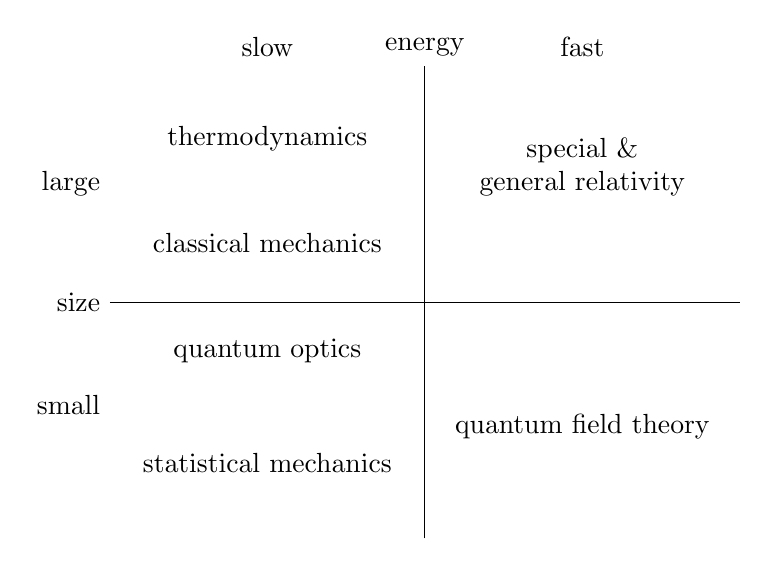
\begin{tikzpicture}
        \draw (-4,0) node[anchor=east] {size} -- (4,0);
        \draw (0,-3) -- (0,3) node[anchor=south] {energy};
        \draw[white] (-2.1,3) -- (-1.9,3) node[black,midway,anchor=south] {slow};
        \draw[white] (1.9,3) -- (2.1,3) node[black,midway,anchor=south] {fast};
        \draw[white] (-4,1.5) node[black,anchor=east] {large} -- (-3.9,1.5);
        \draw[white] (-4,-1.3) node[black,anchor=east] {small} -- (-3.9,-1.3);
        \draw[white] (-2.1,-0.35) -- (-1.9,-0.35) node[black,midway,anchor=north,align=center] {quantum optics};
        \draw[white] (-2.1,-1.8) -- (-1.9,-1.8) node[black,midway,anchor=north,align=center] {statistical mechanics};
        \draw[white] (-2.1,1.8) -- (-1.9,1.8) node[black,midway,anchor=south,align=center] {thermodynamics};
        \draw[white] (1.9,2.2) -- (2.1,2.2) node[black,midway,anchor=north,align=center] {\shortstack{special \&\\general relativity}};
        \draw[white] (1.9,-1.3) -- (2.1,-1.3) node[black,midway,anchor=north,align=center] {quantum field theory};
        \draw[white] (-2.1,0.5) -- (-1.9,0.5) node[black,midway,anchor=south,align=center] {classical mechanics};
    \end{tikzpicture}
\end{figure}

\textbf{Ingredients:}
\begin{itemize}
    \item harmonic oscillators
    \item Gaussian integrals
    \item Hamiltonian mechanics (canonical variables q and p)
    \item maths of operators - adjoint, self-adjoint, Hermitian, commutation relations
    \item QM in both Schrodinger and Heisenberg pictures
    \item density matrices
    \item classical EM - Maxwell's equations in Coulomb gauge - especially plane waves and dipoles
\end{itemize}

Hanbury Brown and Tiss:
\begin{equation}
    G(\tau) = I_A(t)I_B(t+\tau)
\end{equation}

\chapter{}
\section{Learning Outcomes}
To be able to state, explain and apply the operator formalism of the quantum harmonic oscillator to stuff

\section{Quantum Harmonic Oscillator}
\begin{align}
    F &= ma = m\ddot{x} \\
      &= -kx \\
    x(t) &= x_0\sin\om t \\
    p_x(t) &= p_0\cos\om t \\
    V(x) &= \frac12 kx^2 = \frac12 m\om^2x^2 \\
    \frac{\hbar^2}{2m}\frac{d^2\psi}{dx^2} &+ V(x)\psi(x) = E\psi \\
    E_n &= \left(n+\frac12\right)\hbar\om
\end{align}
   
\begin{figure}[H]
    \centering
    \begin{tikzpicture}
        \draw[->,thick] (-3,0) -- (3,0) node[anchor=south] {$x$};
        \draw[->,thick] (0,-0.3) -- (0,2) node[anchor=south] {$V(x)$};
        \draw (0,0) parabola (2.5,1.8);
        \draw (0,0) parabola (-2.5,1.8);
    \end{tikzpicture}
\end{figure}
Start with writing the Hamiltonian, then turn everything into operators
\begin{align}
    H &= \frac{p^2}{2m} + \underbrace{\frac12 m\om^2x^2}_{V(x)} \\
    p &\to \hp = -i\hbar\frac{d}{dx},~ x \to \hx \\
    [\hx,\hp] &= i\hbar \\
    H &= \frac{\hp^2}{2m} + \frac12m\om^2\hx^2 \\
    \ha &= \frac{1}{\sqrt{2m\hbar\om}}\left(m\om\hx+i\hp\right) \\
    \hag &= \frac{1}{\sqrt{2m\hbar\om}} \left(m\om\hx - i\hp\right) \\
    \hx &= \left(\frac{\hbar}{2m\om}\right)^{1/2}(\ha+\hag) \\
    \hp &= -i\left(\frac{m\hbar\om}{2}\right)^{1/2}(\ha-\hag) \\
    [\ha,\hag] &= \ha\hag - \hag\ha = 1 \\
    \hh &= \hbar\om(\hag\ha+\frac12) \\
    \hag\ha &= \hn,~ \hn|n\rangle = n|n\rangle \\
    \hh|n\rangle &= \hbar\om\left(n+\frac12\right)|n\rangle = E_n|n\rangle
\end{align}
How do the annihilation and creation operators, $\ha$ and $\hag$ interact with the number states, $|n\rangle$?
\begin{align}
    \hag|n\rangle &= \sqrt{n+1}|n+1\rangle \\
    \ha|n\rangle &= \sqrt|n-1\rangle
\end{align}
Together, the creation and annihilation operators are known as the \textit{ladder operators.}
Ladder operators move the system up or down the energy levels of the harmonic potential.
\begin{figure}[H]
    \centering
    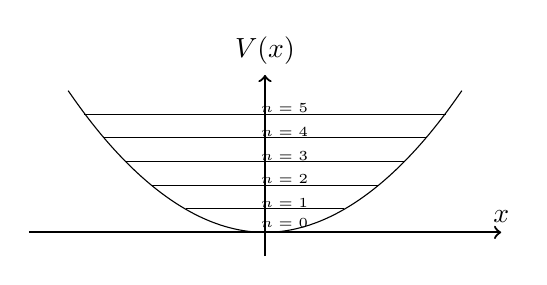
\begin{tikzpicture}
        \draw[->,thick] (-3,0) -- (3,0) node[anchor=south] {$x$} node[anchor=south,midway,xshift=7pt,yshift=-2pt] {\tiny $n=0$};
        \draw[->,thick] (0,-0.3) -- (0,2) node[anchor=south] {$V(x)$};
        \draw (0,0) parabola (2.5,1.8);
        \draw (0,0) parabola (-2.5,1.8);
        \draw (-2.3,1.5) -- (2.3,1.5) node[anchor=south,midway,xshift=7pt,yshift=-3pt] {\tiny $n=5$};
        \draw (-2.05,1.2) -- (2.05,1.2) node[anchor=south,midway,xshift=7pt,yshift=-3pt] {\tiny $n=4$};
        \draw (-1.78,0.9) -- (1.78,0.9) node[anchor=south,midway,xshift=7pt,yshift=-3pt] {\tiny $n=3$};
        \draw (-1.45,0.6) -- (1.45,0.6) node[anchor=south,midway,xshift=7pt,yshift=-3pt] {\tiny $n=2$};
        \draw (-1,0.3) -- (1,0.3) node[anchor=south,midway,xshift=7pt,yshift=-3pt] {\tiny $n=1$};
    \end{tikzpicture}
\end{figure}
We now have a partly new mathematical representation. 
Notice that the potential still remains positive, it does not go negative.
Therefore we must have:
\begin{align}
    \ha|0\rangle &= 0, \\
    \hn &= \hag\ha|0\rangle = 0. \\
    \implies \hh|0\rangle &= E_0|0\rangle = \frac12\hbar\om|0\rangle
\end{align}
So the ground state is labelled '0' but does not have $E=0$.\\
Now we introduce $\hog$ as the adjoint of $\ho$ if
\begin{align}
    \langle\psi|\ho|\phi\rangle &= \langle\phi|\hog|\psi\rangle^*\; \forall \psi,\phi
\end{align}
A self-adjoint operator is equivalent to a Hermitian operator, i.e. $\hn, \hh$.\\
For adjoint operators:
\begin{align}
    (\hat{A}+\hat{B})^\dagger &= \hat{A}^\dagger + \hat{B}^\dagger \\
    (\hat{A}\hat{B})^\dagger &= \hat{B}^\dagger\hat{A}^\dagger \\
    (c\hat{A})^\dagger &+ c^*\hat{A}^\dagger \\
    (\hat{A}^\dagger)^\dagger &= \hat{A}
\end{align}
More on the number states:
\begin{itemize}
    \item they are orthogonal
        \begin{align}
            \langle n|n\rangle &= 1 \\
            \langle n|m\rangle &= 0,~ n\neq m \\
            \langle n|m\rangle &= \delta_{n,m} \\
        \end{align}
    \item they form a basis (note: not mathematically a Hilbert space, but a Banah(?) space)
        \begin{align}
            |\psi\rangle &= \sum_n c_n|n\rangle \\
            0 &\leq n \leq \infty
        \end{align}
\end{itemize}

\section{Two Oscillators - independent}
\begin{align}
    |\psi_0\rangle &= \sum_n c_n|n\rangle_0 \\
    |\psi_1\rangle &= \sum_m c_m|m\rangle_1 \\
    |\psi_{01}\rangle &= \sum_{n,m} c_{n,m}|n\rangle_0|m\rangle_1
\end{align}
What we are doing is "tensoring" the Hilbert spaces: $\mathcal{H}_0 \otimes \mathcal{H}_1$:
\begin{align}
    |n\rangle_0|m\rangle_1 &\equiv |n\rangle_0\otimes|m\rangle_1.
\end{align}
Now we have the operators, $\ha_0,\hag_0,\ha_1,\hag_1$:
\begin{align}
    \ha_0 \otimes \mathbb{I}_1&,~ \mathbb{I}_0\otimes \ha_1,\dots \\
    [\ha_0,\ha_1] &= [\ha_0,\hag_1] = 0 \\
    \hh &= \hh_0\otimes\mathbb{I}_1 + \mathbb{I}_1\otimes\hh_1 
\end{align}
Note this is for non-interacting oscillators. 
For interacting, 
\begin{align}
    \hh &= \hh_0\otimes\mathbb{I}_1 + \mathbb{I}_1\otimes\hh_1 + \mathcal{H}_{int}.
\end{align}


\end{document}


















